\section{Test of the developed components}

\begin{wrapfigure}[19]{L}{0.43\textwidth}
    \vspace{-\baselineskip}
    \centering
     \begin{minipage}[b]{0.39\textwidth}
         \centering
         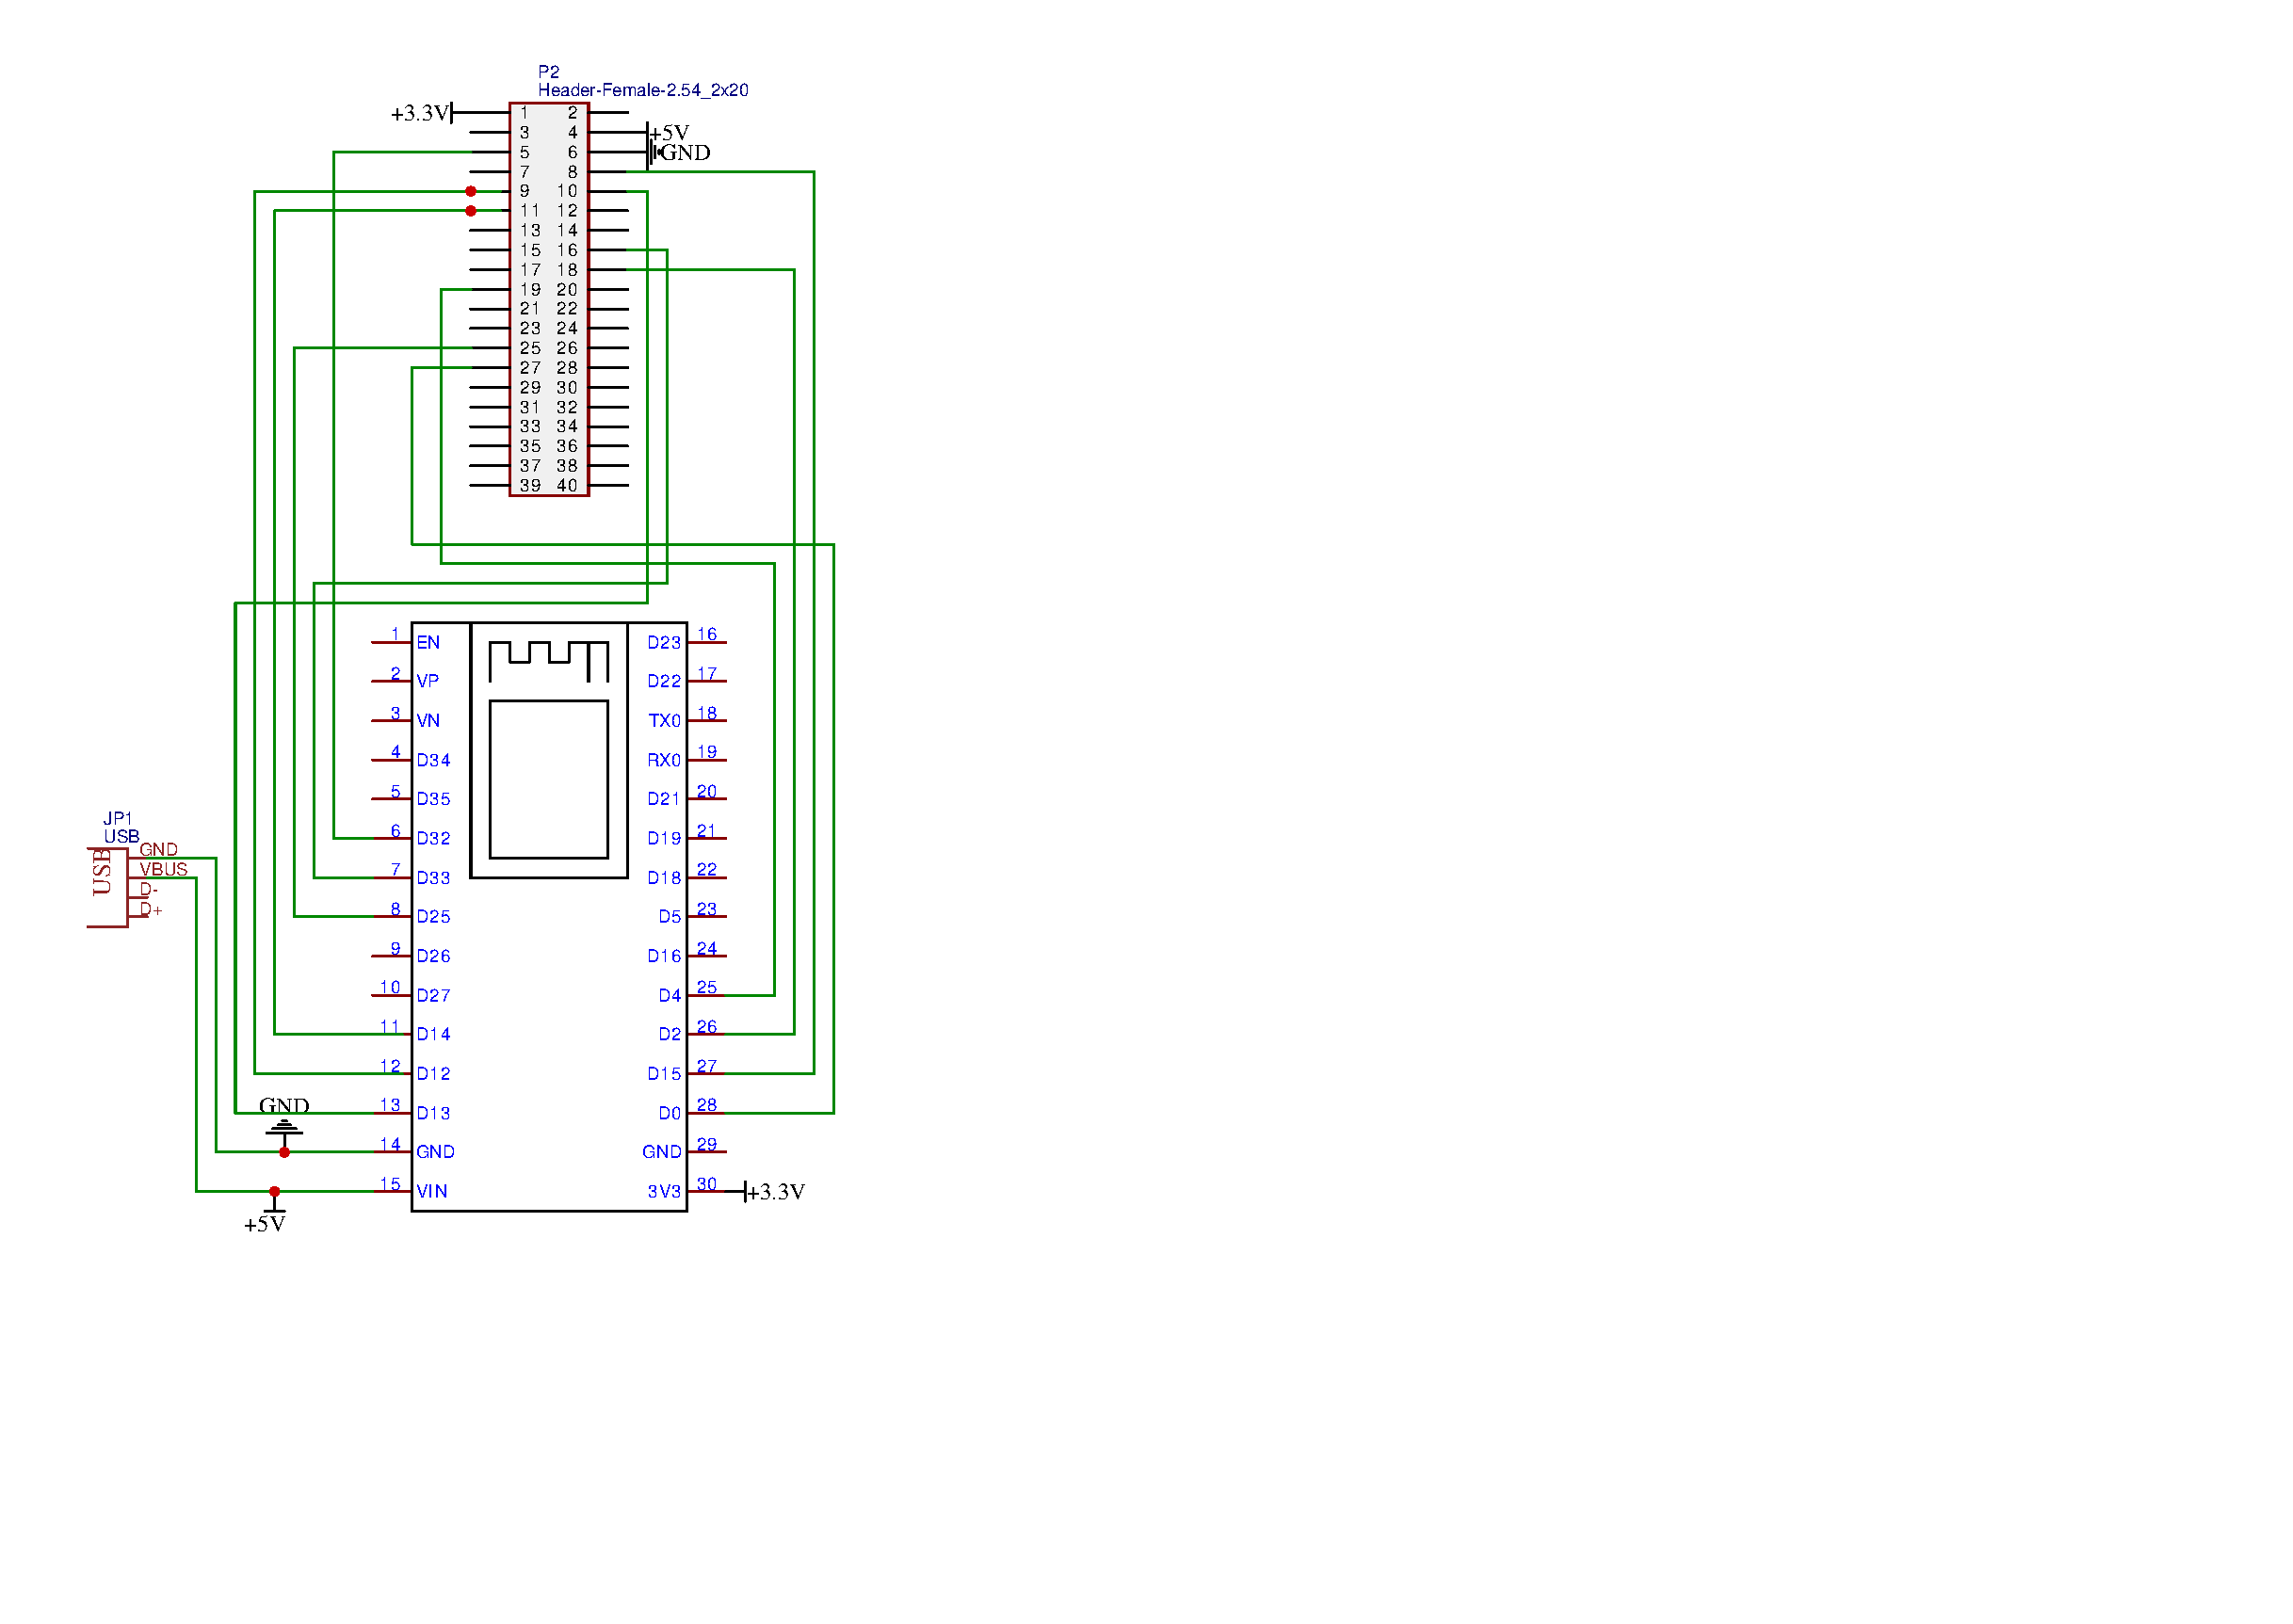
\includegraphics[width=\textwidth]{images/4_2/schmatic_project.pdf}
         \caption{Electrical diagram}
         \label{fig:schem_electronics}
     \end{minipage}
     \vspace{-.25\baselineskip}
\end{wrapfigure}

In this chapter, the conceptual design of chapter \ref{concept} is used. It must be considered that only systems and routines that have been implemented in all three components, i.e. in the frontend, in the backend and in the AS-Pair, will be presented.\\

One can see in figure \ref{fig:schem_electronics} the electronic connections drawn from the ESP32 to the Raspberry GPIO interface of the RWU board.\\

\vspace{4cm}

\begin{listing}[H]
    \begin{minted}[frame=single,
                   framesep=3mm,
                   linenos=true,
                   xleftmargin=21pt,
                   tabsize=3]{json}
{
    "name": "Love_Ship",
    "protocol": {
			"name": "MQTT",
			"specifications": {
				"broker": "192.168.4.1",
				"main_topic": "garden/lab"
			}
		}
}
    \end{minted}
    \vspace{-4mm}
    \caption{Adding an AS-Pair} 
    \label{list:adding_pair}
\end{listing}